\documentclass[oneside,english,11pt]{article}
\usepackage[
    a4paper,
    left=1in,
    right=1in,
    top=0.9in,
    bottom=0.9in,
    headsep=0.3in
]{geometry}


\usepackage[T1]{fontenc}
\usepackage{amsmath}
\usepackage{amssymb}
\usepackage{amsfonts}
\usepackage{mathtools}
\usepackage{graphicx}
\usepackage{booktabs}
\usepackage{array}
\usepackage{longtable}
\usepackage{float}
\usepackage{placeins}
\usepackage{caption}
\usepackage{natbib}
\usepackage{hyperref}
\usepackage{microtype}
\usepackage{ragged2e}
\usepackage{enumitem}
\usepackage{xcolor}
\usepackage{titlesec}
\usepackage{tikz}
\usetikzlibrary{arrows.meta,calc,positioning}


\renewcommand{\boxed}[1]{#1}
\AtBeginDocument{\justifying}


\setlength{\parindent}{0pt}
\setlength{\parskip}{3pt plus 1pt minus 1pt}
\setlength{\abovedisplayskip}{7pt plus 2pt minus 2pt}
\setlength{\belowdisplayskip}{7pt plus 2pt minus 2pt}
\setlength{\abovedisplayshortskip}{4pt plus 1pt minus 1pt}
\setlength{\belowdisplayshortskip}{5pt plus 1pt minus 1pt}
\setlength{\jot}{4pt}
\renewcommand{\arraystretch}{1.15}
\setlength{\textfloatsep}{12pt}
\setlength{\intextsep}{10pt}
\setlist[itemize]{topsep=4pt,itemsep=2pt,parsep=0pt}
\setlist[enumerate]{topsep=4pt,itemsep=2pt,parsep=0pt}
\titlespacing*{\section}{0pt}{12pt}{6pt}
\titlespacing*{\subsection}{0pt}{9pt}{4pt}
\linespread{1.03}
\emergencystretch=2em

\graphicspath{{figures/}}

\captionsetup{
    font=small,
    labelfont=bf,
    justification=centering
}

\newcommand{\lecture}[3]{
    \begin{center}
        \fbox{
            \begin{minipage}{0.94\textwidth}
                \centering

                \vspace{3mm}

                {\bfseries
                IE 643: Deep Learning - Theory and Practice}

                \hfill

                {\small July-Nov 2026}

                \vspace{5mm}

                {\Large\bfseries Project Report}

                \vspace{3mm}

                {\large\bfseries #1}

                \vspace{5mm}

                {\bfseries Team: #2}

                \vspace{2mm}

                {\bfseries Student: #3}

                \vspace{3mm}
            \end{minipage}
        }
    \end{center}

    \vspace{6mm}
}


\begin{document}

\lecture
{Comparing Topological Early-Warning Signals vs.
Classical Volatility Indicators for Predicting Market Crashes}
{AXIOM}
{Dipendu Pal (25N0465)}


\begin{abstract}

This project investigates whether topological features derived from financial returns can improve the prediction of significant market declines. Using daily closing prices from four major US stock indices, I construct rolling point clouds based on joint log returns.

Vietoris-Rips persistent homology (dimensions zero and one) is applied to extract persistence summaries and persistence-landscape features, which are compared to 18 classical financial indicators.

The prediction target is defined as an S\&P 500 decline of at least 10\% within the next 30 trading days.

Models trained include logistic regression, LSTM, bidirectional LSTM, and Transformer architectures, using chronological data splits and three different topological window sizes.

The combined-feature LSTM achieves a mean test average precision of 0.2459 across three random seeds, compared to 0.1340 for the classical-only LSTM.

However, the combined model exhibits weaker validation performance, so I do not claim that topological features consistently enhance prediction in all market periods.

This report presents the mathematical methods, implementation details, experimental results, and study limitations.

\end{abstract}


\section{Introduction}

Sharp declines in stock markets can have profound consequences for investors and financial institutions. 

Accurately forecasting such events remains difficult, given the ever-changing market environment and the infrequency of crashes. 

Standard risk metrics like volatility and recent returns are frequently employed, but they offer only a limited perspective because they do not account for the intricate, joint behavior of several indices.



In this project, each trading day is mapped to a point in a four-dimensional return space, and a rolling window of these points creates a dynamic point cloud. 

Topological Data Analysis (TDA) examines how connected components and loops in this cloud emerge and vanish as the distance threshold changes.

I assess whether summary statistics derived from these topological features can enhance a classifier's ability to anticipate forthcoming market crashes.



The primary objective is to compare the predictive effectiveness of classical features, TDA features, and their combination for a unified crash-prediction task. 

Additionally, I evaluate the performance of a basic linear classifier alongside three neural network architectures to test the robustness and generalizability of the results.

\section{Project Workflow}
\label{sec:workflow}

The main steps in this project are as follows:

\begin{enumerate}[leftmargin=*]

\item Define the prediction target as an S\&P 500 decline of at least 10\% within the next 30 trading days.

\item Download and align daily closing prices for four major US stock indices.

\item Calculate log returns, compute 18 classical financial indicators, and generate forward crash labels.

\item Construct rolling return point clouds using window sizes of 40, 80, and 120 trading days.

\item Compute $H_0$ and $H_1$ persistence diagrams for each point cloud.

\item Transform persistence diagrams into numerical features, including persistence counts, lifetimes, landscape norms, and differences between consecutive landscapes.

\item Train logistic regression, LSTM, bidirectional LSTM, and Transformer models on these features.

\item Repeat all neural network experiments using three different random seeds to assess variability.

\item Compare the predictive value of individual TDA window sizes with the combination of all three windows.

\item Analyze the behavior of indicators around historical market crashes.

\item Save trained models and reload a checkpoint for a historical prediction demonstration.

\end{enumerate}



\section{Related Work}

\label{sec:related}

\subsection{Persistent Homology}

Edelsbrunner, Letscher, and Zomorodian \citep{edelsbrunner2002} explored how to compute topological persistence.

They developed a mathematical framework to track how topological features appear and fade away as we adjust a scale parameter. This framework underpins the persistent-homology features I use in my project.


\subsection{Persistence Landscapes}

Bubenik \citep{bubenik2015} introduced persistence landscapes as a functional representation of persistence diagrams.

For this project, I used persistence-landscape norms and the step-to-step changes in those landscapes as input features to help make predictions.


\subsection{Topological Features in Financial Markets}

Gidea and Katz \citep{gidea2018} studied topological signatures of financial-market instability.


\subsection{Persistent Homology as an Early-Warning Signal}

Ismail et al. \citep{ismail2022} studied the use of persistent homology for detecting early-warning signals of financial crises.

Their research got me thinking-do shifts in topological features line up with times when the financial markets get shaky?
To explore that, I set up a simple crash-prediction task and compared these topological features with regular financial indicators.


\subsection{Classical Early-Warning Indicators}

Diks, Hommes, and Wang \citep{diks2019} studied critical slowing down as a possible early-warning signal for financial crises.

Critical slowing down means a system bounces back more slowly from bumps in the road as it approaches a big change.
That’s why it makes sense to look at how statistical signals change before the market gets rocky.
In my project, I used classical financial indicators as a starting point to see if topological features add any extra predictive power.

\subsection{Deep Learning for Sequential Data}

Hochreiter and Schmidhuber \citep{hochreiter1997} introduced Long Short-Term Memory networks.

LSTMs have gates that decide what information to keep or toss as data moves through a sequence. This setup helps them learn patterns over time.
In my work, I used an LSTM to find connections between past financial data and whether a crash happened later.


Vaswani et al. \citep{vaswani2017} introduced the Transformer architecture, which uses attention to model relationships between sequence positions.

Transformers work differently than recurrent models-they use self-attention to look at all parts of a sequence at once, instead of passing information step by step.
I added a Transformer encoder to see how attention-based models stack up against the LSTM and BiLSTM approaches.



\subsection{How My Project Differs from Previous Work}

The foundational literature informs this project's methodology. 

Persistent homology serves to reveal structural patterns within financial return point clouds, and persistence landscapes convert these topological insights into quantitative features.

Classical early-warning indicators provide a baseline, summarizing shifts in financial market behaviour through established statistical measures.

Deep learning models are employed to uncover and learn intricate temporal patterns present in sequences of these various indicators.

In this project, I integrate these concepts and conduct the following comparisons:

\begin{enumerate}

\item Classical financial indicators alone.

\item Topological features alone.

\item  Combined classical and topological features.

\item LSTM, bidirectional LSTM, and Transformer models.

\item TDA features calculated using rolling windows of 40, 80, and 120 days.

\end{enumerate}

The central question is whether topological features contribute additional predictive value beyond classical financial indicators.

This is evaluated using chronologically split training, validation, and test datasets to avoid look-ahead bias.

The analysis also examines the behavior of both indicator types around historical market crashes, providing insights into their responsiveness and utility as early-warning signals.

The objective is not to assert that TDA consistently surpasses classical methods, but to identify the circumstances in which it proves advantageous, those in which it does not, and how its predictive performance measures up against established simpler approaches.

\section{Methods and Approaches}
\label{sec:methods}

\subsection{Work Before the Preparation Review}

The initial plan was to compare classical financial-risk
indicators with features obtained using persistent homology.

The main steps were to define a market-crash prediction
problem, identify the financial indices, study persistent
homology, and design a pipeline for extracting topological
features from rolling windows.

\subsection{Work After the Preparation Review}

After the preparation review, I implemented the complete
data-processing and training pipeline.

I added persistence-landscape summaries, multiple
window sizes, logistic-regression baselines, three
neural-network architectures, repeated runs with different
random seeds, and a window-size ablation.

I also generated historical market-crash plots and
a saved-checkpoint prediction demonstration.

\subsection{Daily Log Returns}

Let $P_t^{(j)}$ denote the closing price of index $j$
on trading day $t$.

The daily log return is

\begin{equation}
\boxed{
r_t^{(j)}
=
\log\left(
\frac{P_t^{(j)}}{P_{t-1}^{(j)}}
\right).
}
\end{equation}

This can also be written as

\begin{equation}
r_t^{(j)}
=
\log P_t^{(j)}
-
\log P_{t-1}^{(j)}.
\end{equation}

Log returns are useful because returns over consecutive
periods can be added.

For example,

\begin{align}
r_t+r_{t-1}
&=
\log\left(\frac{P_t}{P_{t-1}}\right)
+
\log\left(\frac{P_{t-1}}{P_{t-2}}\right)
\\
&=
\log\left(\frac{P_t}{P_{t-2}}\right).
\end{align}

\subsection{Four-Dimensional Return Vectors}

I use four stock indices.

For each trading day, I construct

\begin{equation}
\boxed{
X_t=
\begin{bmatrix}
r_t^{(1)}\\
r_t^{(2)}\\
r_t^{(3)}\\
r_t^{(4)}
\end{bmatrix}
\in\mathbb{R}^4.
}
\end{equation}

Thus, each trading day becomes a point in
four-dimensional Euclidean space.

\subsection{Rolling Point Clouds}

For a window of length $w$, the point cloud ending
on day $t$ is

\begin{equation}
\boxed{
\mathcal{X}_t^{(w)}
=
\left\{
X_{t-w+1},
X_{t-w+2},
\ldots,
X_t
\right\}.
}
\end{equation}

I use three window sizes:

\begin{equation}
w\in\{40,80,120\}.
\end{equation}

For example, when $w=40$, the point cloud contains
40 points in $\mathbb{R}^4$.

The implementation multiplies log returns by 100
before computing persistent homology.

This converts decimal log returns into
percentage-point units.

\subsection{Euclidean Distance}

For two return vectors $X_i,X_j\in\mathbb{R}^4$,
the Euclidean distance is

\begin{equation}
\boxed{
d(X_i,X_j)
=
\sqrt{
\sum_{k=1}^{4}
\left(
X_i^{(k)}-X_j^{(k)}
\right)^2
}.
}
\end{equation}

These distances are used to construct the
Vietoris-Rips filtration.

\subsection{Basic Geometric Ideas}

Before defining the Vietoris-Rips complex, I first
explain the basic geometric objects used in its
construction.

A simplex is a basic building block of a
simplicial complex.

A 0-simplex is a point.

A 1-simplex is an edge joining two points.

A 2-simplex is a filled triangle.

A 3-simplex is a filled tetrahedron.

Figure~\ref{fig:simplices} shows these four objects.

\begin{figure}[htbp]
\centering

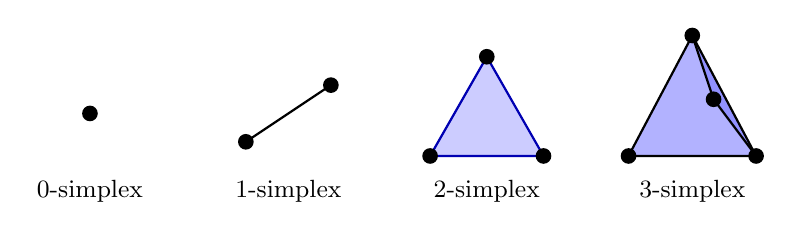
\begin{tikzpicture}[
    scale=0.9,
    every node/.style={font=\small},
    vertex/.style={
        circle,
        fill=black,
        inner sep=2pt
    }
]


\begin{scope}[shift={(0,0)}]

\node[vertex] at (0,0.8) {};

\node at (0,-0.3) {0-simplex};

\end{scope}



\begin{scope}[shift={(2.8,0)}]

\draw[thick] (-0.6,0.4) -- (0.6,1.2);

\node[vertex] at (-0.6,0.4) {};
\node[vertex] at (0.6,1.2) {};

\node at (0,-0.3) {1-simplex};

\end{scope}



\begin{scope}[shift={(5.6,0)}]

\filldraw[
    fill=blue!20,
    draw=blue!70!black,
    thick
]
(-0.8,0.2) --
(0.8,0.2) --
(0,1.6) -- cycle;

\node[vertex] at (-0.8,0.2) {};
\node[vertex] at (0.8,0.2) {};
\node[vertex] at (0,1.6) {};

\node at (0,-0.3) {2-simplex};

\end{scope}



\begin{scope}[shift={(8.5,0)}]

\coordinate (A) at (-0.9,0.2);
\coordinate (B) at (0.9,0.2);
\coordinate (C) at (0.3,1.0);
\coordinate (D) at (0,1.9);


\draw[dashed,gray] (A) -- (C);


\fill[blue!12] (A) -- (B) -- (C) -- cycle;
\fill[blue!30] (A) -- (B) -- (D) -- cycle;
\fill[blue!50,opacity=0.65]
(B) -- (C) -- (D) -- cycle;


\draw[thick] (A) -- (B) -- (C);
\draw[thick] (A) -- (D);
\draw[thick] (B) -- (D);
\draw[thick] (C) -- (D);

\node[vertex] at (A) {};
\node[vertex] at (B) {};
\node[vertex] at (C) {};
\node[vertex] at (D) {};

\node at (0,-0.3) {3-simplex};

\end{scope}

\end{tikzpicture}

\caption{
Examples of simplices.
A 0-simplex is a point,
a 1-simplex is an edge,
a 2-simplex is a filled triangle,
and a 3-simplex is a filled tetrahedron.
}

\label{fig:simplices}

\end{figure}


\subsection{Connected Components and Holes}

A connected component is a group of vertices
in which any two vertices can be joined by
a path of edges.

For example, two separate groups of connected
vertices form two connected components.

A one-dimensional hole is represented by a
closed loop that is not the boundary of a
filled region.

The number of connected components is
denoted by $\beta_0$.

The number of independent one-dimensional
holes is denoted by $\beta_1$.

Figure~\ref{fig:betti_examples} illustrates
these ideas.

\begin{figure}[htbp]
\centering

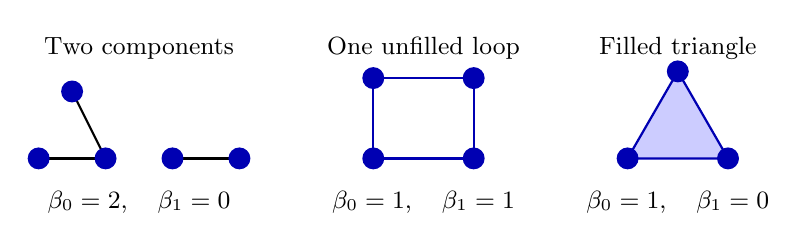
\begin{tikzpicture}[
    scale=0.85,
    vertex/.style={
        circle,
        fill=blue!70!black,
        inner sep=2.8pt
    },
    every node/.style={font=\small}
]


\begin{scope}[shift={(0,0)}]

\draw[thick] (0,0) -- (1,0);
\draw[thick] (1,0) -- (0.5,1);

\node[vertex] at (0,0) {};
\node[vertex] at (1,0) {};
\node[vertex] at (0.5,1) {};

\draw[thick] (2,0) -- (3,0);

\node[vertex] at (2,0) {};
\node[vertex] at (3,0) {};

\node at (1.5,-0.65)
{$\beta_0=2,\quad\beta_1=0$};

\node at (1.5,1.65)
{Two components};

\end{scope}



\begin{scope}[shift={(5,0)}]

\draw[
    thick,
    blue!70!black
]
(0,0) -- (1.5,0) --
(1.5,1.2) -- (0,1.2) -- cycle;

\node[vertex] at (0,0) {};
\node[vertex] at (1.5,0) {};
\node[vertex] at (1.5,1.2) {};
\node[vertex] at (0,1.2) {};

\node at (0.75,-0.65)
{$\beta_0=1,\quad\beta_1=1$};

\node at (0.75,1.65)
{One unfilled loop};

\end{scope}



\begin{scope}[shift={(8.8,0)}]

\filldraw[
    fill=blue!20,
    draw=blue!70!black,
    thick
]
(0,0) -- (1.5,0) --
(0.75,1.3) -- cycle;

\node[vertex] at (0,0) {};
\node[vertex] at (1.5,0) {};
\node[vertex] at (0.75,1.3) {};

\node at (0.75,-0.65)
{$\beta_0=1,\quad\beta_1=0$};

\node at (0.75,1.65)
{Filled triangle};

\end{scope}

\end{tikzpicture}

\caption{
Examples of connected components and
one-dimensional holes.
An unfilled loop contributes to $H_1$,
while the boundary of a filled triangle
does not.
}

\label{fig:betti_examples}

\end{figure}

\noindent
These examples show the difference between
a closed path and a topological hole.

A closed path does not always produce a
nonzero first homology class.

If the path is the boundary of a filled
region, it represents zero in $H_1$.

\subsection{Vietoris-Rips Complex}

Let $(X,d)$ be a finite metric space.

For a scale parameter $\varepsilon\geq0$,
the Vietoris-Rips complex is

\begin{equation}
\boxed{
VR_{\varepsilon}(X)
=
\left\{
\sigma\subseteq X:
d(x_i,x_j)\leq\varepsilon
\text{ for every }x_i,x_j\in\sigma
\right\}.
}
\end{equation}

A simplex is included when all pairs of its vertices
are within distance $\varepsilon$.

For example, two points form an edge when their
distance is at most $\varepsilon$.

Three points form a filled triangle when all
three pairwise distances are at most $\varepsilon$.

\subsection{Filtration}

If

\begin{equation}
\varepsilon_1\leq\varepsilon_2,
\end{equation}

then

\begin{equation}
\boxed{
VR_{\varepsilon_1}(X)
\subseteq
VR_{\varepsilon_2}(X).
}
\end{equation}

To see this, suppose a simplex $\sigma$ belongs to
$VR_{\varepsilon_1}(X)$.

By definition, every pair of vertices satisfies

\begin{equation}
d(x_i,x_j)\leq\varepsilon_1.
\end{equation}

Since $\varepsilon_1\leq\varepsilon_2$,

\begin{equation}
d(x_i,x_j)\leq\varepsilon_2.
\end{equation}

Therefore, the same simplex also belongs to
$VR_{\varepsilon_2}(X)$.

This proves the inclusion.

A nested collection of such complexes is called
a filtration.

\subsection{Example: Vietoris-Rips Filtration
of a Square}

Consider four points at the corners of a
unit square:

\begin{equation}
A=(0,0),\quad
B=(1,0),\quad
C=(1,1),\quad
D=(0,1).
\end{equation}

The distance between neighbouring vertices
is 1.

The distance between opposite vertices
is $\sqrt{2}$.

I now increase the distance threshold
$\varepsilon$ and observe how the
Vietoris-Rips complex changes.

\begin{figure}[htbp]
\centering

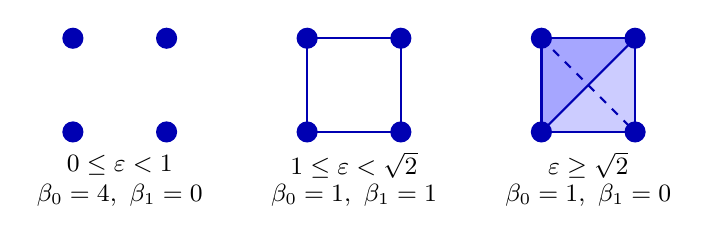
\begin{tikzpicture}[
    scale=0.85,
    vertex/.style={
        circle,
        fill=blue!70!black,
        inner sep=2.7pt
    },
    every node/.style={font=\small}
]


\begin{scope}[shift={(0,0)}]

\node[vertex] at (0,0) {};
\node[vertex] at (1.4,0) {};
\node[vertex] at (1.4,1.4) {};
\node[vertex] at (0,1.4) {};

\node at (0.7,-0.5)
{$0\leq\varepsilon<1$};

\node at (0.7,-0.95)
{$\beta_0=4,\ \beta_1=0$};

\end{scope}



\begin{scope}[shift={(3.5,0)}]

\draw[
    thick,
    blue!70!black
]
(0,0) -- (1.4,0) --
(1.4,1.4) -- (0,1.4) -- cycle;

\node[vertex] at (0,0) {};
\node[vertex] at (1.4,0) {};
\node[vertex] at (1.4,1.4) {};
\node[vertex] at (0,1.4) {};

\node at (0.7,-0.5)
{$1\leq\varepsilon<\sqrt{2}$};

\node at (0.7,-0.95)
{$\beta_0=1,\ \beta_1=1$};

\end{scope}



\begin{scope}[shift={(7,0)}]


\fill[blue!20]
(0,0) -- (1.4,0) --
(1.4,1.4) -- cycle;

\fill[blue!35]
(0,0) -- (1.4,1.4) --
(0,1.4) -- cycle;


\draw[
    thick,
    blue!70!black
]
(0,0) -- (1.4,0) --
(1.4,1.4) -- (0,1.4) -- cycle;


\draw[
    thick,
    blue!70!black
]
(0,0) -- (1.4,1.4);

\draw[
    thick,
    dashed,
    blue!70!black
]
(0,1.4) -- (1.4,0);

\node[vertex] at (0,0) {};
\node[vertex] at (1.4,0) {};
\node[vertex] at (1.4,1.4) {};
\node[vertex] at (0,1.4) {};

\node at (0.7,-0.5)
{$\varepsilon\geq\sqrt{2}$};

\node at (0.7,-0.95)
{$\beta_0=1,\ \beta_1=0$};

\end{scope}

\end{tikzpicture}

\caption{
Vietoris-Rips filtration of four points
at the corners of a unit square.
As the distance threshold increases,
four isolated components merge into one,
a loop appears, and the loop is later filled.
At the final stage, the complex contains
the full 3-simplex on the four vertices;
the drawing shows its two-dimensional faces.
}

\label{fig:vr_square}

\end{figure}


\paragraph{Stage 1: Four Isolated Points.}

When $0\leq\varepsilon<1$, no edges
are present.

The complex contains four isolated
vertices.

Therefore,

\begin{equation}
\beta_0=4,\qquad\beta_1=0.
\end{equation}


\paragraph{Stage 2: Formation of a Loop.}

At $\varepsilon=1$, the four edges
of the square appear.

All vertices become connected.

However, the interior is not filled.

Therefore,

\begin{equation}
\beta_0=1,\qquad\beta_1=1.
\end{equation}

The one-dimensional hole is born at

\begin{equation}
b=1.
\end{equation}


\paragraph{Stage 3: The Loop Disappears.}

At $\varepsilon=\sqrt{2}$, both
diagonal edges appear.

All pairwise distances between the
four vertices are now at most
$\varepsilon$.

Therefore, the Vietoris-Rips
complex contains the full 3-simplex
on these four vertices.

Its triangular faces fill the
previous square loop.

Thus,

\begin{equation}
\beta_0=1,\qquad\beta_1=0.
\end{equation}

The loop dies at

\begin{equation}
d=\sqrt{2}.
\end{equation}

Its persistence is

\begin{equation}
\ell=d-b=\sqrt{2}-1\approx0.4142.
\end{equation}

This example shows how persistent
homology records the birth and death
of topological features.

\subsection{Homology}

Homology is an algebraic method for studying
topological features.

I calculate homology in dimensions zero and one.

The group $H_0$ describes connected components.

The group $H_1$ describes independent one-dimensional
loops that are not boundaries of filled regions.

Let $C_k$ be the vector space generated by
the $k$-dimensional simplices.

The boundary operator is

\begin{equation}
\partial_k:C_k\longrightarrow C_{k-1}.
\end{equation}

For an oriented simplex,

\begin{equation}
[v_0,v_1,\ldots,v_k],
\end{equation}

the boundary is

\begin{equation}
\boxed{
\partial_k[v_0,\ldots,v_k]
=
\sum_{i=0}^{k}
(-1)^i
[v_0,\ldots,\widehat{v_i},\ldots,v_k].
}
\end{equation}

The symbol $\widehat{v_i}$ means that vertex $v_i$
is omitted.

The boundary operators satisfy

\begin{equation}
\boxed{
\partial_{k-1}\circ\partial_k=0.
}
\end{equation}

Define the cycle space as

\begin{equation}
Z_k=\ker(\partial_k)
\end{equation}

and the boundary space as

\begin{equation}
B_k=\operatorname{im}(\partial_{k+1}).
\end{equation}

The $k$-th homology group is

\begin{equation}
\boxed{
H_k=Z_k/B_k.
}
\end{equation}

Its dimension is called the $k$-th Betti number:

\begin{equation}
\boxed{
\beta_k=\dim H_k.
}
\end{equation}

\subsection{Persistent Homology}

Ordinary homology studies a complex at one scale.

Persistent homology tracks homology classes
as the filtration scale changes.

A persistent feature is represented by a
birth-death pair

\begin{equation}
(b_i,d_i),
\end{equation}

where $b_i$ is the scale at which the feature
appears and $d_i$ is the scale at which it disappears.

The persistence of the feature is

\begin{equation}
\boxed{
\ell_i=d_i-b_i.
}
\end{equation}

A persistence diagram is the multiset

\begin{equation}
\boxed{
D_k=
\left\{
(b_i,d_i)
\right\}_{i=1}^{m_k}.
}
\end{equation}

For every rolling window, I calculate the
$H_0$ and $H_1$ persistence diagrams.

The implementation uses Ripser with
maximum homology dimension equal to one.

\subsection{Example: Persistence Diagram}

A persistence diagram represents each
topological feature by a point $(b,d)$,
where $b$ is its birth scale and
$d$ is its death scale.

For the square example, the loop is born
at $\varepsilon=1$ and dies at
$\varepsilon=\sqrt{2}$.

Therefore, the corresponding point in
the first persistence diagram is

\begin{equation}
(b,d)=(1,\sqrt{2}).
\end{equation}

\begin{figure}[htbp]
\centering

\begin{tikzpicture}[
    scale=3,
    >=Stealth
]


\draw[->,thick]
(0,0) -- (1.8,0)
node[right] {$b$};

\draw[->,thick]
(0,0) -- (0,1.8)
node[above] {$d$};


\draw[
    dashed,
    gray,
    thick
]
(0,0) -- (1.65,1.65);

\node[
    gray,
    rotate=45,
    font=\scriptsize
]
at (0.6,0.7) {$d=b$};


\filldraw[
    fill=blue!70!black,
    draw=blue!70!black
]
(1,1.4142) circle (0.035);


\draw[
    red!70!black,
    thick,
    <-> 
]
(1.12,1) -- (1.12,1.4142);

\node[
    right,
    font=\scriptsize
]
at (1.14,1.2)
{$\sqrt{2}-1$};


\draw[dotted]
(1,0) -- (1,1.4142);

\draw[dotted]
(0,1.4142) -- (1,1.4142);


\node[below,font=\scriptsize]
at (1,0) {$1$};

\node[left,font=\scriptsize]
at (0,1.4142) {$\sqrt{2}$};

\node[
    above left,
    font=\scriptsize
]
at (1,1.4142)
{$(1,\sqrt{2})$};

\end{tikzpicture}

\caption{
The $H_1$ persistence diagram for the
unit-square example.
The point $(1,\sqrt{2})$ represents
the loop that appears at scale 1
and disappears at scale $\sqrt{2}$.
The vertical segment shows its persistence
$\sqrt{2}-1$.
}

\label{fig:persistence_square}

\end{figure}

\noindent
A point closer to the diagonal has
a smaller persistence value.

A point farther above the diagonal
has a larger persistence value.

However, a larger persistence value
does not automatically mean that the
corresponding feature is useful for
predicting a financial crash.

\subsection{Persistence Landscapes}

A persistence diagram may contain a different
number of points for different rolling windows.

To obtain numerical features with a fixed size,
I use persistence landscapes.

For a birth-death interval $(b_i,d_i)$,
define the triangular function

\begin{equation}
\boxed{
f_i(x)
=
\max\left\{
0,
\min(x-b_i,d_i-x)
\right\}.
}
\end{equation}

Equivalently,

\begin{equation}
f_i(x)=
\begin{cases}
0,
& x<b_i,
\\
x-b_i,
& b_i\leq x\leq\dfrac{b_i+d_i}{2},
\\
d_i-x,
& \dfrac{b_i+d_i}{2}<x\leq d_i,
\\
0,
& x>d_i.
\end{cases}
\end{equation}

The function reaches its maximum at

\begin{equation}
x=\frac{b_i+d_i}{2}.
\end{equation}

The maximum height is

\begin{equation}
\boxed{
\max_x f_i(x)
=
\frac{d_i-b_i}{2}.
}
\end{equation}

At every value of $x$, the triangular functions
are sorted in decreasing order.

The $k$-th persistence landscape is defined by

\begin{equation}
\boxed{
\lambda_k(x)
=
\text{$k$-th largest value of }
\{f_i(x)\}_{i=1}^{m}.
}
\end{equation}

I retain the first five landscape layers.

The functions are evaluated numerically using
160 grid points.

\subsection{Landscape $L^1$ Norm}

The $L^1$ norm of the retained landscape layers is

\begin{equation}
\boxed{
\|\lambda\|_1
=
\sum_{k=1}^{5}
\int_{\mathbb{R}}
|\lambda_k(x)|\,dx.
}
\end{equation}

Since persistence landscapes are nonnegative,

\begin{equation}
\|\lambda\|_1
=
\sum_{k=1}^{5}
\int_{\mathbb{R}}
\lambda_k(x)\,dx.
\end{equation}

This measures the total area under the retained
landscape layers.

For one persistence interval of length

\begin{equation}
\ell=d-b,
\end{equation}

the triangular function has base length $\ell$
and height $\ell/2$.

Therefore,

\begin{align}
\int_{\mathbb{R}}f(x)\,dx
&=
\frac{1}{2}
\times\ell
\times\frac{\ell}{2}
\\
&=
\boxed{\frac{\ell^2}{4}}.
\end{align}

\subsection{Landscape $L^2$ Norm}

The $L^2$ norm is

\begin{equation}
\boxed{
\|\lambda\|_2
=
\left(
\sum_{k=1}^{5}
\int_{\mathbb{R}}
\lambda_k(x)^2\,dx
\right)^{1/2}.
}
\end{equation}

For a single triangular function with persistence
$\ell$, symmetry gives

\begin{align}
\int_{\mathbb{R}}f(x)^2\,dx
&=
2\int_0^{\ell/2}u^2\,du
\\
&=
2\left[
\frac{u^3}{3}
\right]_0^{\ell/2}
\\
&=
\frac{\ell^3}{12}.
\end{align}

Hence,

\begin{equation}
\boxed{
\|f\|_2
=
\sqrt{\frac{\ell^3}{12}}.
}
\end{equation}

This explains why longer persistence intervals
can contribute strongly to the $L^2$ norm.

\subsection{Other Persistence Summaries}

For a persistence diagram $D$, total persistence is

\begin{equation}
\boxed{
TP(D)
=
\sum_{i=1}^{m}(d_i-b_i).
}
\end{equation}

Maximum persistence is

\begin{equation}
\boxed{
MP(D)
=
\max_i(d_i-b_i).
}
\end{equation}

I also calculate the number of finite
persistence intervals.

For $n$ distinct points, the finite $H_0$
interval count is normally $n-1$.

Therefore, the corresponding counts for
40, 80, and 120 day windows are

\begin{equation}
39,\qquad79,\qquad119.
\end{equation}

These constant features are excluded from
model training.

\subsection{Persistence-Landscape Change}

Let $\lambda_{t,k}^{(w)}$ be the $k$-th
$H_1$ persistence-landscape layer for the
window ending at time $t$.

I calculate the change between consecutive
landscapes as

\begin{equation}
\boxed{
\Delta_t^{(w)}
=
\left[
\sum_{k=1}^{5}
\int_{\mathbb{R}}
\left(
\lambda_{t,k}^{(w)}(x)
-
\lambda_{t-1,k}^{(w)}(x)
\right)^2dx
\right]^{1/2}.
}
\end{equation}

A larger value indicates a greater change
between the two landscape representations.

This does not automatically mean that a
market crash will follow.

\subsection{Feature Construction}

For each window, I calculate five finite
persistence summaries for $H_0$:

\begin{itemize}
\item Number of finite intervals.
\item Total persistence.
\item Maximum persistence.
\item Landscape $L^1$ norm.
\item Landscape $L^2$ norm.
\end{itemize}

I calculate the same five summaries for $H_1$,
together with the $H_1$ landscape-change feature.

Thus, each window produces

\begin{equation}
5+5+1=11
\end{equation}

raw TDA features.

With three windows,

\begin{equation}
3\times11=33.
\end{equation}

After removing three constant $H_0$ count
features, the TDA feature set contains

\begin{equation}
\boxed{30\text{ features}.}
\end{equation}

The classical feature set contains 18 features.

The combined representation therefore contains

\begin{equation}
\boxed{
18+30=48\text{ features}.
}
\end{equation}

\subsection{Crash Prediction Target}

Let $P_t$ denote the S\&P 500 closing price.

The binary target is

\begin{equation}
\boxed{
Y_t=
\mathbf{1}
\left\{
\min_{1\leq h\leq30}
P_{t+h}
\leq0.9P_t
\right\}.
}
\end{equation}

Here, $\mathbf{1}\{\cdot\}$ denotes the
indicator function.

Thus, $Y_t=1$ when the S\&P 500 falls
by at least 10\% relative to its closing
price on day $t$ at some point during
the next 30 trading days.

Otherwise,

\begin{equation}
Y_t=0.
\end{equation}

\subsection{Logistic Regression}

Logistic regression is used as a baseline.

For a feature vector $x$, the predicted
probability is

\begin{equation}
\boxed{
P(Y=1\mid x)
=
\frac{1}{
1+\exp[-(\beta_0+\beta^\top x)]
}.
}
\end{equation}

The model assumes that the log-odds are linear:

\begin{equation}
\log\left(
\frac{p}{1-p}
\right)
=
\beta_0+\beta^\top x.
\end{equation}

Solving for $p$ gives the logistic function.

I train separate baseline models using
classical, TDA, and combined features.

\subsection{Deep Learning Input}

For each prediction date $t$, the neural network
receives 30 consecutive feature vectors.

If $z_t\in\mathbb{R}^{p}$ is the feature vector
on day $t$, then

\begin{equation}
\boxed{
Z_t=
\begin{bmatrix}
z_{t-29}\\
z_{t-28}\\
\vdots\\
z_t
\end{bmatrix}
\in\mathbb{R}^{30\times p}.
}
\end{equation}

The sequence length is 30.

The feature dimension depends on whether
classical, TDA, or combined features are used.

\subsection{Long Short-Term Memory Network}

An LSTM processes a sequence while maintaining
a hidden state and a cell state.

Let $x_t$ be the input at sequence step $t$.

The forget gate is

\begin{equation}
\boxed{
f_t=
\sigma(W_fx_t+U_fh_{t-1}+b_f).
}
\end{equation}

The input gate is

\begin{equation}
\boxed{
i_t=
\sigma(W_ix_t+U_ih_{t-1}+b_i).
}
\end{equation}

The candidate cell state is

\begin{equation}
\boxed{
\widetilde{c}_t
=
\tanh(W_cx_t+U_ch_{t-1}+b_c).
}
\end{equation}

The output gate is

\begin{equation}
\boxed{
o_t=
\sigma(W_ox_t+U_oh_{t-1}+b_o).
}
\end{equation}

The cell state is updated by

\begin{equation}
\boxed{
c_t=
f_t\odot c_{t-1}
+
i_t\odot\widetilde{c}_t.
}
\end{equation}

The hidden state is

\begin{equation}
\boxed{
h_t=
o_t\odot\tanh(c_t).
}
\end{equation}

Here, $\odot$ represents elementwise multiplication.

The LSTM in my implementation uses a
32-dimensional hidden state.

The final hidden representation is passed
through a linear layer to produce one logit.

\subsection{Bidirectional LSTM}

A bidirectional LSTM processes the available
historical sequence in two directions.

The forward hidden state is

\begin{equation}
\overrightarrow{h}_t
=
F(x_t,\overrightarrow{h}_{t-1}).
\end{equation}

The backward hidden state is

\begin{equation}
\overleftarrow{h}_t
=
B(x_t,\overleftarrow{h}_{t+1}).
\end{equation}

The representations are combined as

\begin{equation}
\boxed{
h_t=
\begin{bmatrix}
\overrightarrow{h}_t\\
\overleftarrow{h}_t
\end{bmatrix}.
}
\end{equation}

Each direction uses 32 hidden units.

Therefore, the combined representation
has dimension 64.

The backward direction does not use
observations after the prediction date.
It only processes the supplied historical
sequence in reverse order.

\subsection{Transformer Encoder}

The Transformer uses self-attention to
model relationships between different
positions in the input sequence.

Given an input representation $X$,
the query, key, and value matrices are

\begin{align}
Q&=XW_Q,\\
K&=XW_K,\\
V&=XW_V.
\end{align}

Scaled dot-product attention is

\begin{equation}
\boxed{
\operatorname{Attention}(Q,K,V)
=
\operatorname{softmax}
\left(
\frac{QK^\top}{\sqrt{d_k}}
\right)V.
}
\end{equation}

The division by $\sqrt{d_k}$ controls
the scale of the dot products.

My Transformer uses:

\begin{itemize}
\item Embedding dimension: 32.
\item Attention heads: 4.
\item Encoder layers: 2.
\item Feedforward dimension: 64.
\item Dropout: 0.15.
\end{itemize}

The final sequence representation is
passed through a linear classifier.

\subsection{Binary Cross-Entropy Loss}

For a binary label $y\in\{0,1\}$
and predicted probability $p$,
binary cross-entropy is

\begin{equation}
\boxed{
\ell(y,p)
=
-y\log p
-
(1-y)\log(1-p).
}
\end{equation}

This is the negative log-likelihood
of a Bernoulli observation.

Because positive crash labels are relatively
rare, I use a weighted loss.

Let $N_+$ and $N_-$ denote the numbers
of positive and negative training examples.

The positive-class weight is

\begin{equation}
\boxed{
w_+=\frac{N_-}{N_+}.
}
\end{equation}

The weighted loss becomes

\begin{equation}
\boxed{
\ell(y,p)
=
-w_+y\log p
-
(1-y)\log(1-p).
}
\end{equation}

The implementation uses
\texttt{BCEWithLogitsLoss}, which combines
the sigmoid transformation and binary
cross-entropy in a numerically stable form.

\subsection{AdamW Optimizer}

I train the neural-network models using
AdamW, an adaptive gradient-based optimiser
with decoupled weight decay
\citep{loshchilov2019}.

AdamW uses exponential moving averages
of the gradients and their squared values.

Let $\theta_t$ denote the model parameters
and $g_t=\nabla_{\theta}\mathcal{L}(\theta_t)$
the gradient of the training loss.

The first and second moment estimates are

\begin{align}
m_t &= \beta_1 m_{t-1}+(1-\beta_1)g_t,\\
v_t &= \beta_2 v_{t-1}+(1-\beta_2)g_t^2.
\end{align}

After bias correction, the parameters
are updated using

\begin{equation}
\theta_{t+1}
=
\theta_t
-
\eta\frac{\hat m_t}
{\sqrt{\hat v_t}+\epsilon}
-
\eta\lambda\theta_t.
\end{equation}

Here, $\eta$ is the learning rate,
$\lambda$ is the weight-decay coefficient,
and $\epsilon$ is a small constant
for numerical stability.

The weight-decay term is applied
separately from the adaptive gradient
update, which distinguishes AdamW
from standard Adam with an
$L^2$ penalty.

In my experiments, I use
$\eta=0.001$ and $\lambda=0.0001$.

I also apply gradient clipping with
a maximum gradient norm of $1.0$
to limit excessively large updates.


\section{Dataset}
\label{sec:data}

\subsection{Data Sources}

I use daily historical closing prices for
the following US stock indices:

\begin{enumerate}
\item S\&P 500.
\item Dow Jones Industrial Average.
\item NASDAQ Composite.
\item Russell 2000.
\end{enumerate}

The data were downloaded from Yahoo Finance.

The downloaded files cover the historical
period from 1990 to 2026.

The four datasets are aligned by trading date.

I kept only the dates where all the needed data were available.

\subsection{Preprocessing}

The main preprocessing steps are:

\begin{enumerate}

\item Read the historical price files.

\item Extract the relevant closing-price series.

\item Align the four indices by date.

\item Calculate daily log returns.

\item Construct classical financial indicators.

\item Generate the future crash labels.

\item Calculate rolling TDA features.

\item Remove observations with unavailable features
or labels.

\end{enumerate}

The classical-feature dataset contains
8,687 labelled observations.

After aligning the classical indicators
with the rolling topological features,
the final combined dataset contains
8,596 labelled observations.

Approximately 6.69\% of the observations
in the combined dataset have positive
crash labels.

This makes the prediction problem
class-imbalanced.

All main model comparisons use the same
aligned dataset so that the different
feature groups are evaluated on the
same trading dates.

\subsection{Chronological Splitting}

The dataset is split chronologically into training, validation, and test periods to respect the time-ordered nature of financial data.

Mixing earlier and later observations would lead to unrealistic evaluation results.

The feature scaler is fitted exclusively on the training data and then applied unchanged to the validation and test sets. 

Because the crash label depends on the subsequent 30 trading days, the final 30 labeled observations before each split boundary are excluded. 

This ensures that training labels do not use future prices from the validation set, and validation labels do not use future prices from the test set.

Validation and test input sequences may still include earlier historical data, as those observations would have been available at the prediction date.


\section{Experiments}
\label{sec:experiments}

\subsection{Feature Groups}

I compare three main feature groups:

\begin{table}[htbp]
\centering
\caption{Feature groups used in the experiments.}
\label{tab:features}

\begin{tabular}{lc}
\toprule
Feature group & Number of features\\
\midrule
Classical & 18\\
TDA & 30\\
Combined & 48\\
\bottomrule
\end{tabular}

\end{table}

\subsection{Models}

The main experiments use:

\begin{itemize}
\item Logistic regression.
\item LSTM.
\item Bidirectional LSTM.
\item Transformer Encoder.
\end{itemize}

Each neural-network architecture is trained
with each of the three feature groups.

\subsection{Training Settings}

The neural-network experiments use the
following settings:

\begin{table}[htbp]
\centering

\caption{Neural-network training settings.}
\label{tab:training}

\begin{tabular}{ll}
\toprule
Parameter & Value\\
\midrule
Sequence length & 30\\
Batch size & 128\\
Maximum epochs & 25\\
Learning rate & 0.001\\
Optimizer & AdamW\\
Weight decay & 0.0001\\
Gradient clipping norm & 1.0\\
Early-stopping patience & 5\\
Random seeds & 42, 123, 2026\\
\bottomrule
\end{tabular}

\end{table}

\subsection{Repeated Experiments}

For the main neural-network comparison,
I use three architectures, three feature
groups, and three random seeds.

Therefore, the number of neural-network
runs is

\begin{equation}
\boxed{
3\times3\times3=27.
}
\end{equation}

Three logistic-regression baselines
are also trained.

Thus, the initial comparison contains

\begin{equation}
\boxed{
27+3=30\text{ runs}.
}
\end{equation}

\subsection{TDA Window-Size Ablation}

I perform an additional experiment
using the LSTM architecture.

The four TDA configurations are:

\begin{table}[htbp]
\centering

\caption{TDA window-size ablation.}
\label{tab:ablation_settings}

\begin{tabular}{ll}
\toprule
Experiment & TDA features\\
\midrule
A & 40-day window\\
B & 80-day window\\
C & 120-day window\\
D & All three windows\\
\bottomrule
\end{tabular}

\end{table}

The three single-window configurations
are trained using three seeds.

This adds nine new runs.

The all-window LSTM was already included
in the main experiments.

Therefore, the total number of
model-training runs is

\begin{equation}
\boxed{
30+9=39.
}
\end{equation}

\subsection{Evaluation Metrics}


I use precision, recall, F1 score,
ROC-AUC, and average precision.

Precision is

\begin{equation}
\boxed{
\operatorname{Precision}
=
\frac{TP}{TP+FP}.
}
\end{equation}

Recall is

\begin{equation}
\boxed{
\operatorname{Recall}
=
\frac{TP}{TP+FN}.
}
\end{equation}

The F1 score is

\begin{equation}
\boxed{
F_1=
\frac{
2\operatorname{Precision}\operatorname{Recall}
}{
\operatorname{Precision}+\operatorname{Recall}
}.
}
\end{equation}

The main metric is average precision (AP),
stored as \texttt{PR\_AUC} in the code.

It is calculated as

\begin{equation}
\boxed{
AP=
\sum_n
(R_n-R_{n-1})P_n,
}
\end{equation}

where $P_n$ and $R_n$ are precision
and recall at successive thresholds.

AP is useful for evaluating models
when positive labels are rare.

\subsection{Hardware and Reproducibility}

I ran the experiments in Python, using PyTorch, scikit-learn, and Ripser.

The configuration files show that I used Google Colab with an NVIDIA Tesla T4 GPU for training.

Software versions were Python 3.13.16 and PyTorch 2.11.0+cu130. The training scripts use CUDA if there’s a compatible GPU; otherwise, they fall back to the CPU.

For the neural network experiments, I tried three random seeds: 42, 123, and 2026. Each training run saves its setup, training history, evaluation scores, predictions, and the trained model file.

I fit the feature scaler using only the training data.

We can reload the trained model and its scaler to make historical predictions.

I picked the best model by comparing average precision scores on the validation set.



\section{Results and Discussion}
\label{sec:results}

\subsection{Main Model Comparison}

Table~\ref{tab:main_results} gives the
mean test results obtained from the
saved experiment files.

\begin{table}[htbp]
\centering
\small

\caption{
Selected test results.
Neural-network AP values are averaged
across three random seeds.
Standard deviations are shown for
the classical and combined LSTM models.
}
\label{tab:main_results}

\begin{tabular}{llcc}
\toprule
Architecture & Features & AP & ROC-AUC\\
\midrule

Logistic & Classical & 0.1645 & 0.8194\\

LSTM & Classical &
$0.1340\pm0.0423$ & 0.7562\\

LSTM & TDA & 0.0877 & 0.6708\\

\textbf{LSTM} &
\textbf{Combined} &
$\mathbf{0.2459\pm0.0604}$ &
\textbf{0.8732}\\

BiLSTM & Combined & 0.1627 & 0.8130\\

Transformer & Combined & 0.1369 & 0.7679\\

\bottomrule
\end{tabular}

\end{table}

The combined-feature LSTM gets
the highest mean test AP among
the main neural-network configurations.

The classical-only LSTM gets
a mean test AP of 0.1340.

The combined LSTM gets 0.2459.

The relative increase is

\begin{equation}
\frac{
0.2459-0.1340
}{
0.1340
}
\times100
\approx83.5\%.
\end{equation}

This is a relative increase in AP,
not an increase of 83.5 percentage points.

But the combined model doesn’t show the 
same benefit when we look at the validation data.

\subsection{Validation and Test Comparison}

\begin{table}[htbp]
\centering

\caption{Mean validation and test average precision.}
\label{tab:validation}

\begin{tabular}{llcc}
\toprule
Model & Features & Validation AP & Test AP\\
\midrule
LSTM & Classical & 0.1106 & 0.1340\\
LSTM & TDA & 0.0425 & 0.0877\\
LSTM & Combined & 0.0690 & 0.2459\\
BiLSTM & Combined & 0.0487 & 0.1627\\
Transformer & Combined & 0.0632 & 0.1369\\
\bottomrule
\end{tabular}

\end{table}

The combined LSTM model does a lot better
on the test period than it does on the
validation period.

This shows its results really depend
on which market period we look at.

So, I can’t say for sure that
TDA features always help
predictions in every period.

\subsection{TDA Window-Size Ablation}

The ablation compares TDA features
from different rolling-window lengths.

\begin{table}[htbp]
\centering

\caption{TDA window-size ablation using LSTM.}
\label{tab:ablation_results}

\begin{tabular}{lcc}
\toprule
TDA window & Mean test AP & Standard deviation\\
\midrule
40 days & 0.0742 & 0.0018\\
80 days & 0.0828 & 0.0325\\
120 days & 0.0762 & 0.0021\\
All windows & \textbf{0.0877} & 0.0077\\
\bottomrule
\end{tabular}

\end{table}

The all-window representation gets the best mean test AP score.

But the gap between this and the 80-day model isn’t very big.

The 80-day model’s performance jumps around quite a bit depending on the random seed.

The all-window model uses more input features, so this experiment does not fully separate
the effect of window size from the effect of input dimensionality.

\begin{figure}[htbp]
\centering

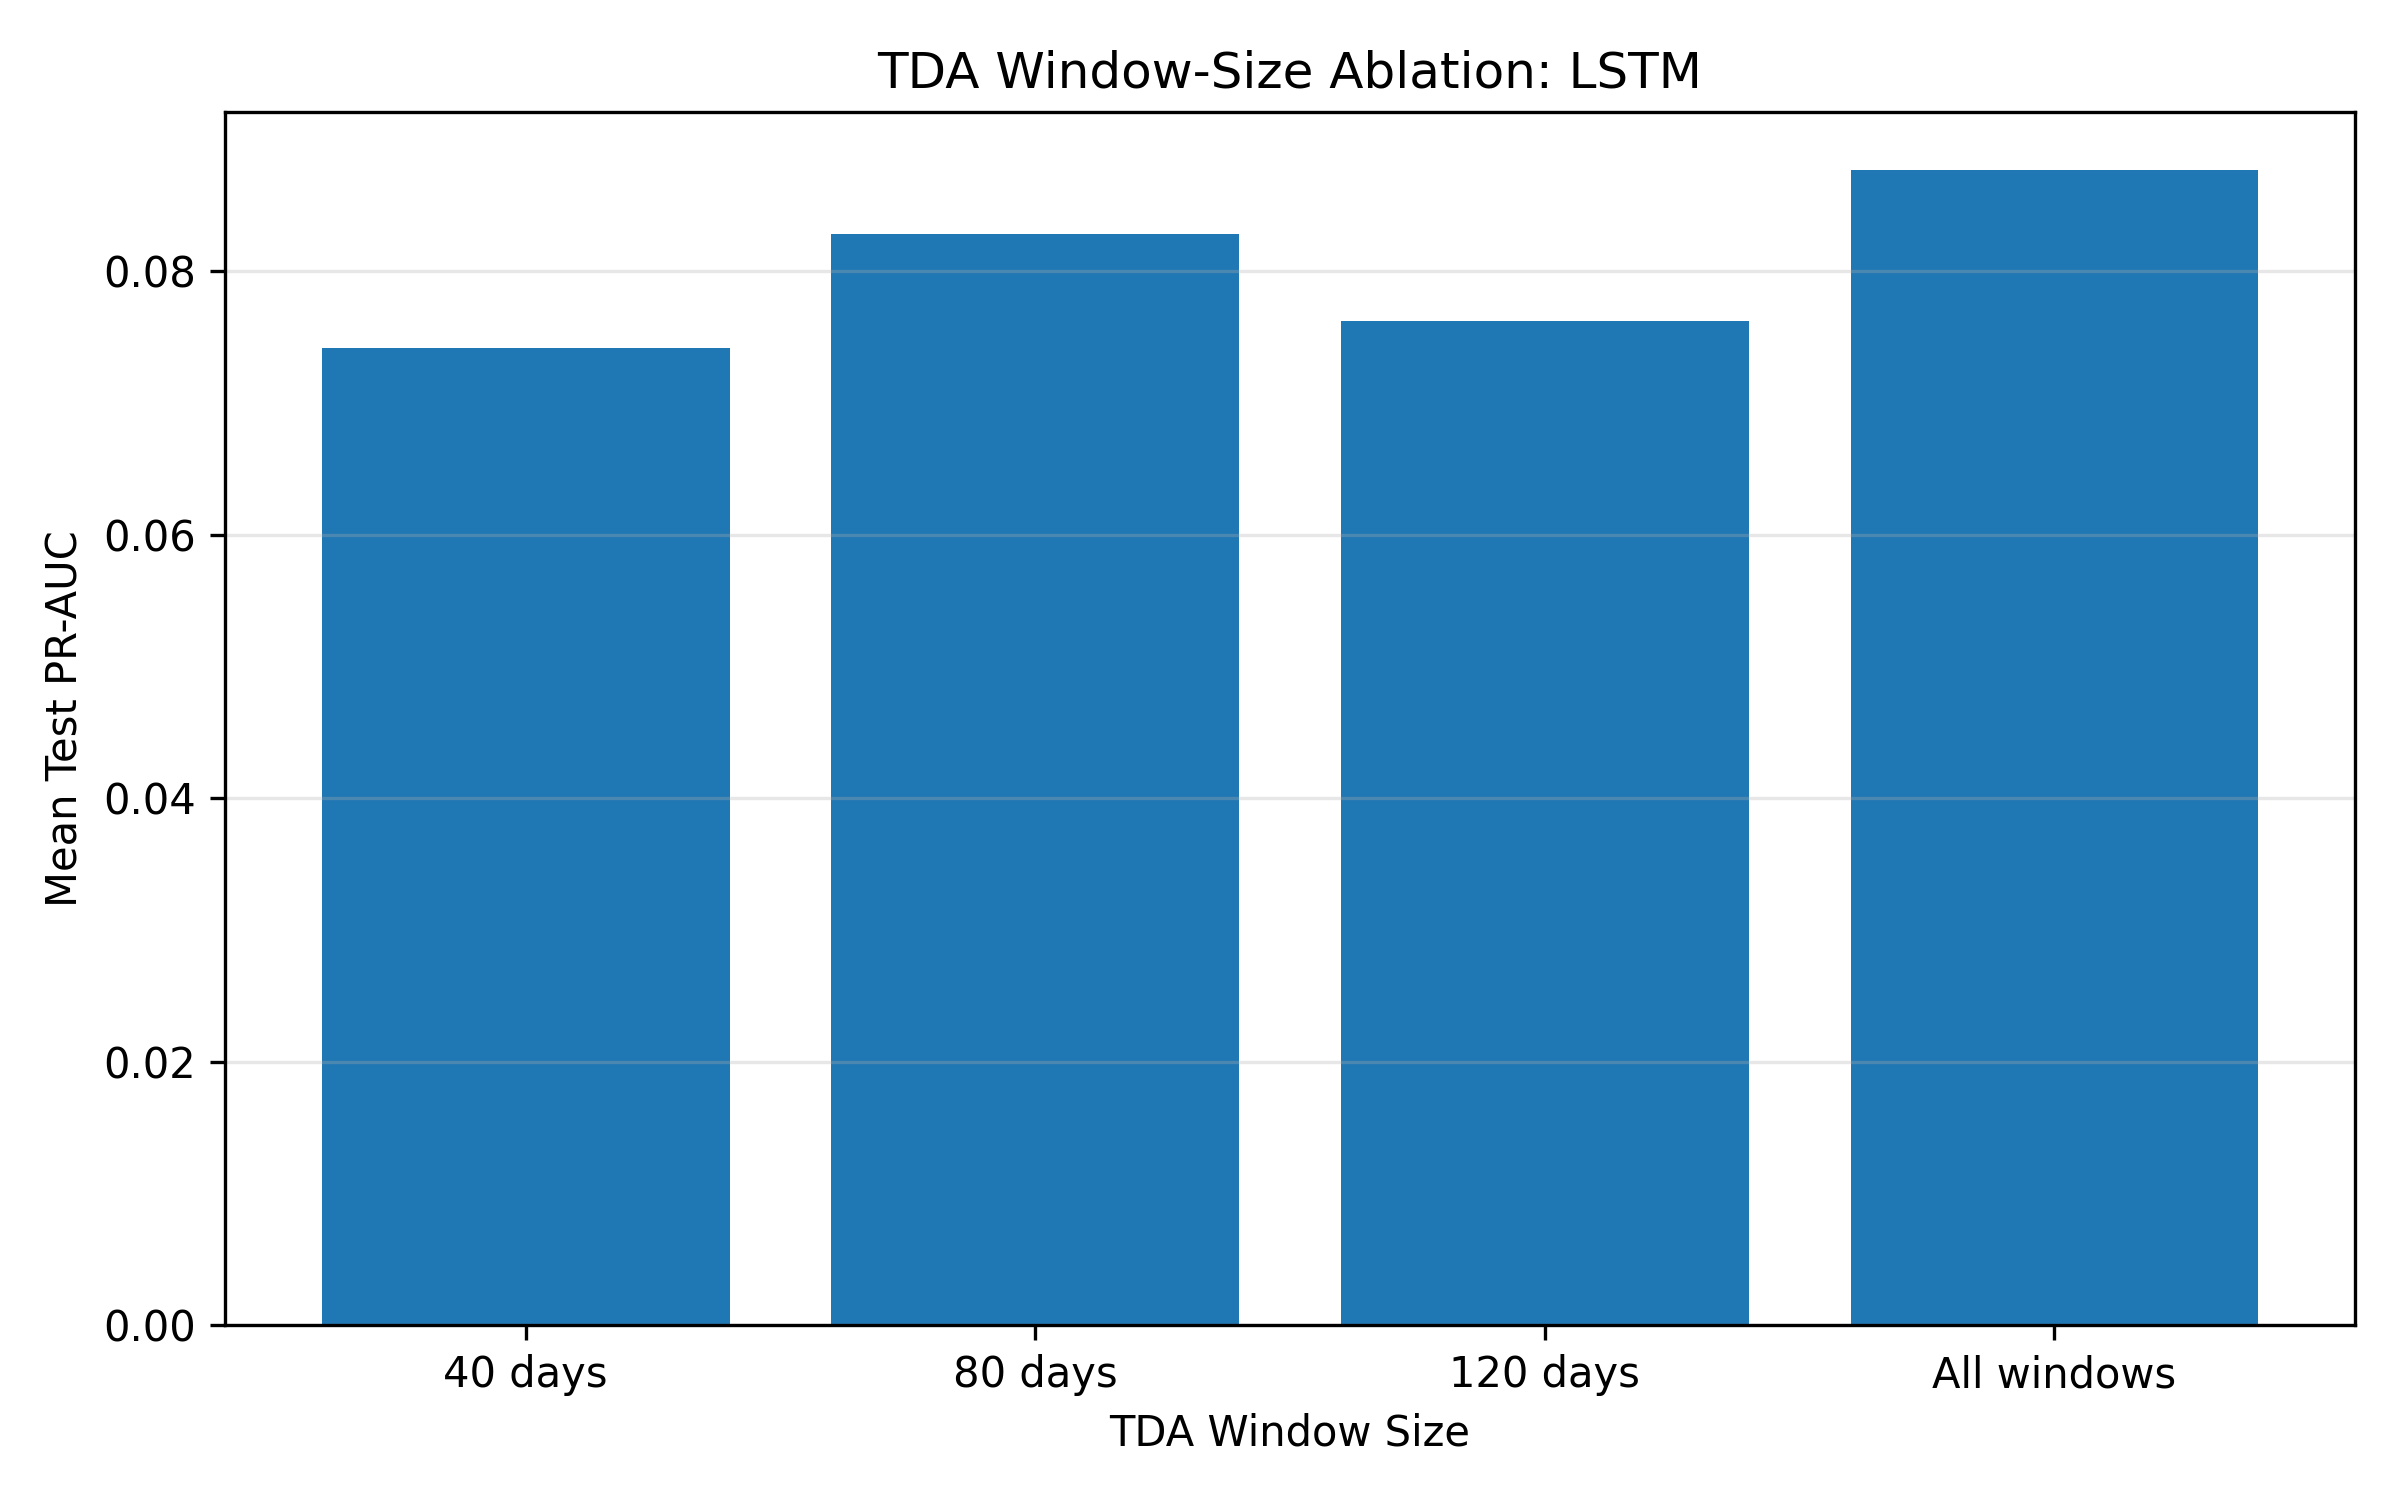
\includegraphics[
    width=0.85\textwidth,
    keepaspectratio
]{tda_window_ablation.png}

\caption{
Mean test average precision for the
TDA window-size ablation using LSTM.
}

\label{fig:tda_ablation}

\end{figure}

\FloatBarrier

\subsection{Historical Market-Crash Analysis}

I wanted to see how typical volatility metrics and certain topological indicators acted during major market declines. Here’s what I looked at:

\begin{itemize}
\item S\&P 500 closing prices.
\item Rolling volatility.
\item $H_1$ persistence-landscape norms.
\item Changes between consecutive landscapes.
\end{itemize}

The charts make it easy to spot shifts in these indicators when the market gets rough. Still, just noticing a spike during a crash doesn’t guarantee these signals are good early warnings.

\begin{figure}[htbp]
\centering

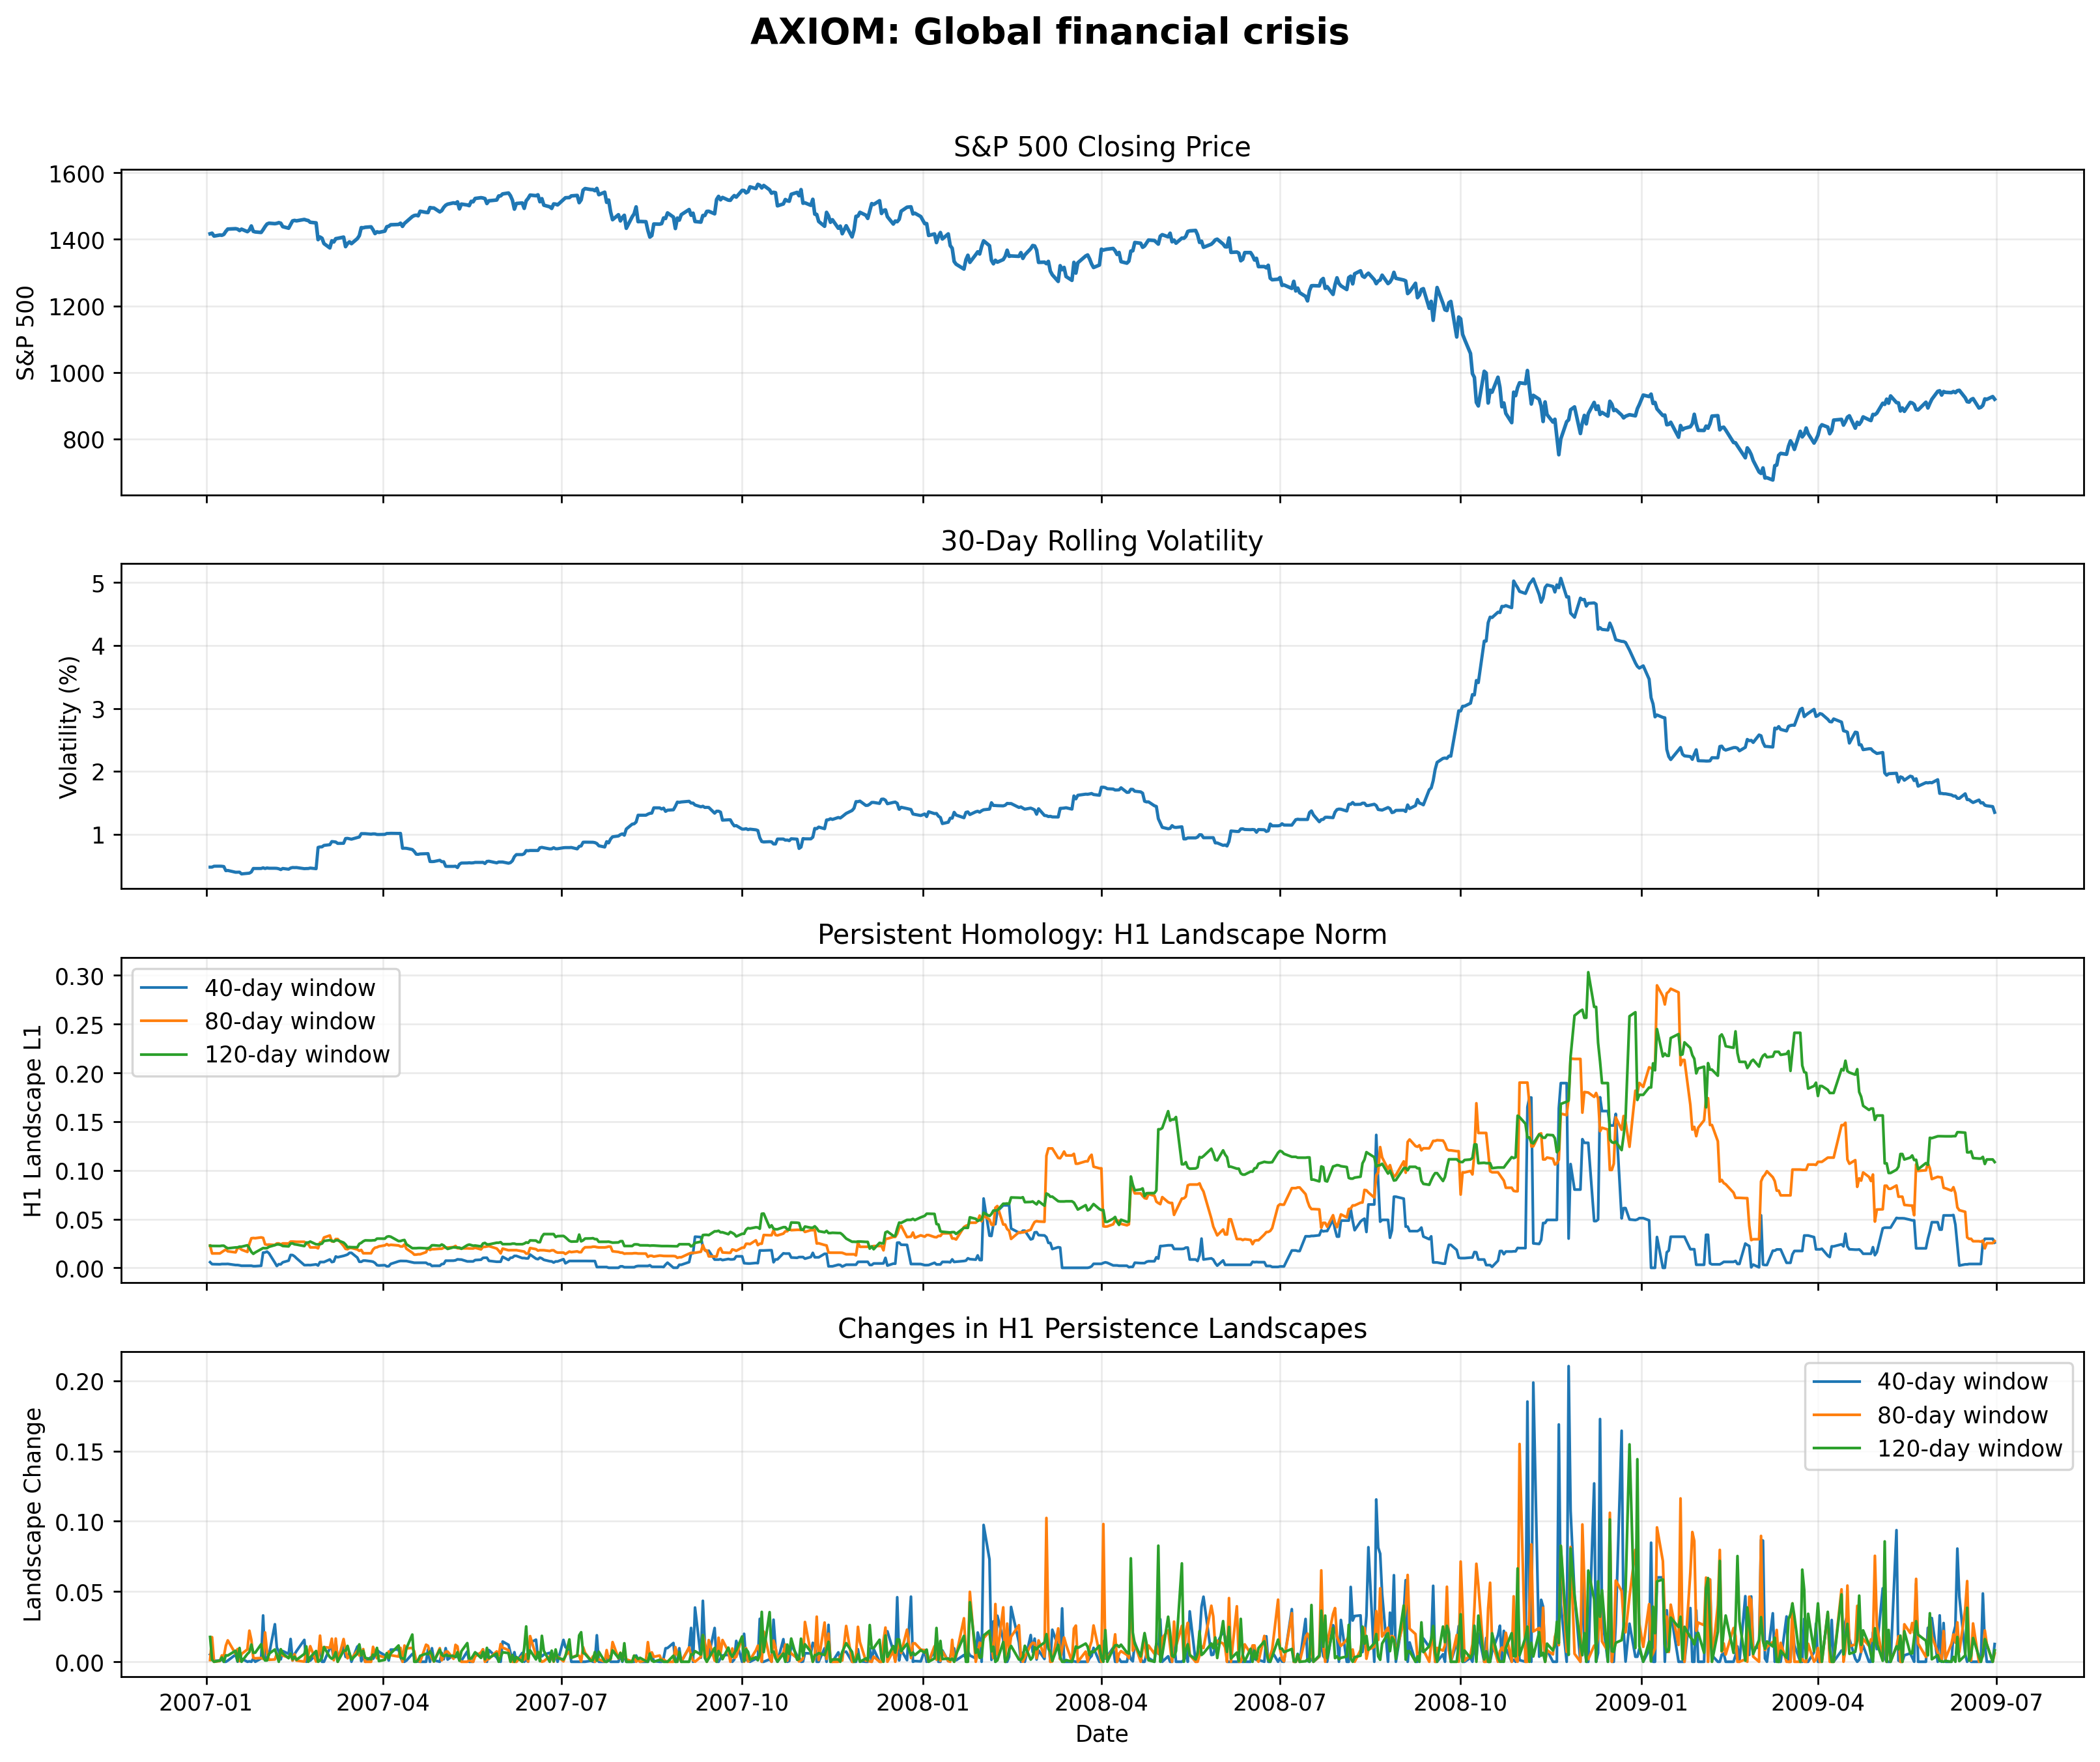
\includegraphics[
    width=0.88\textwidth,
    keepaspectratio
]{global_financial_crisis.png}

\caption{
Classical volatility and topological indicators
around the global financial crisis.
}

\label{fig:financial_crisis}

\end{figure}

\FloatBarrier

\begin{figure}[htbp]
\centering

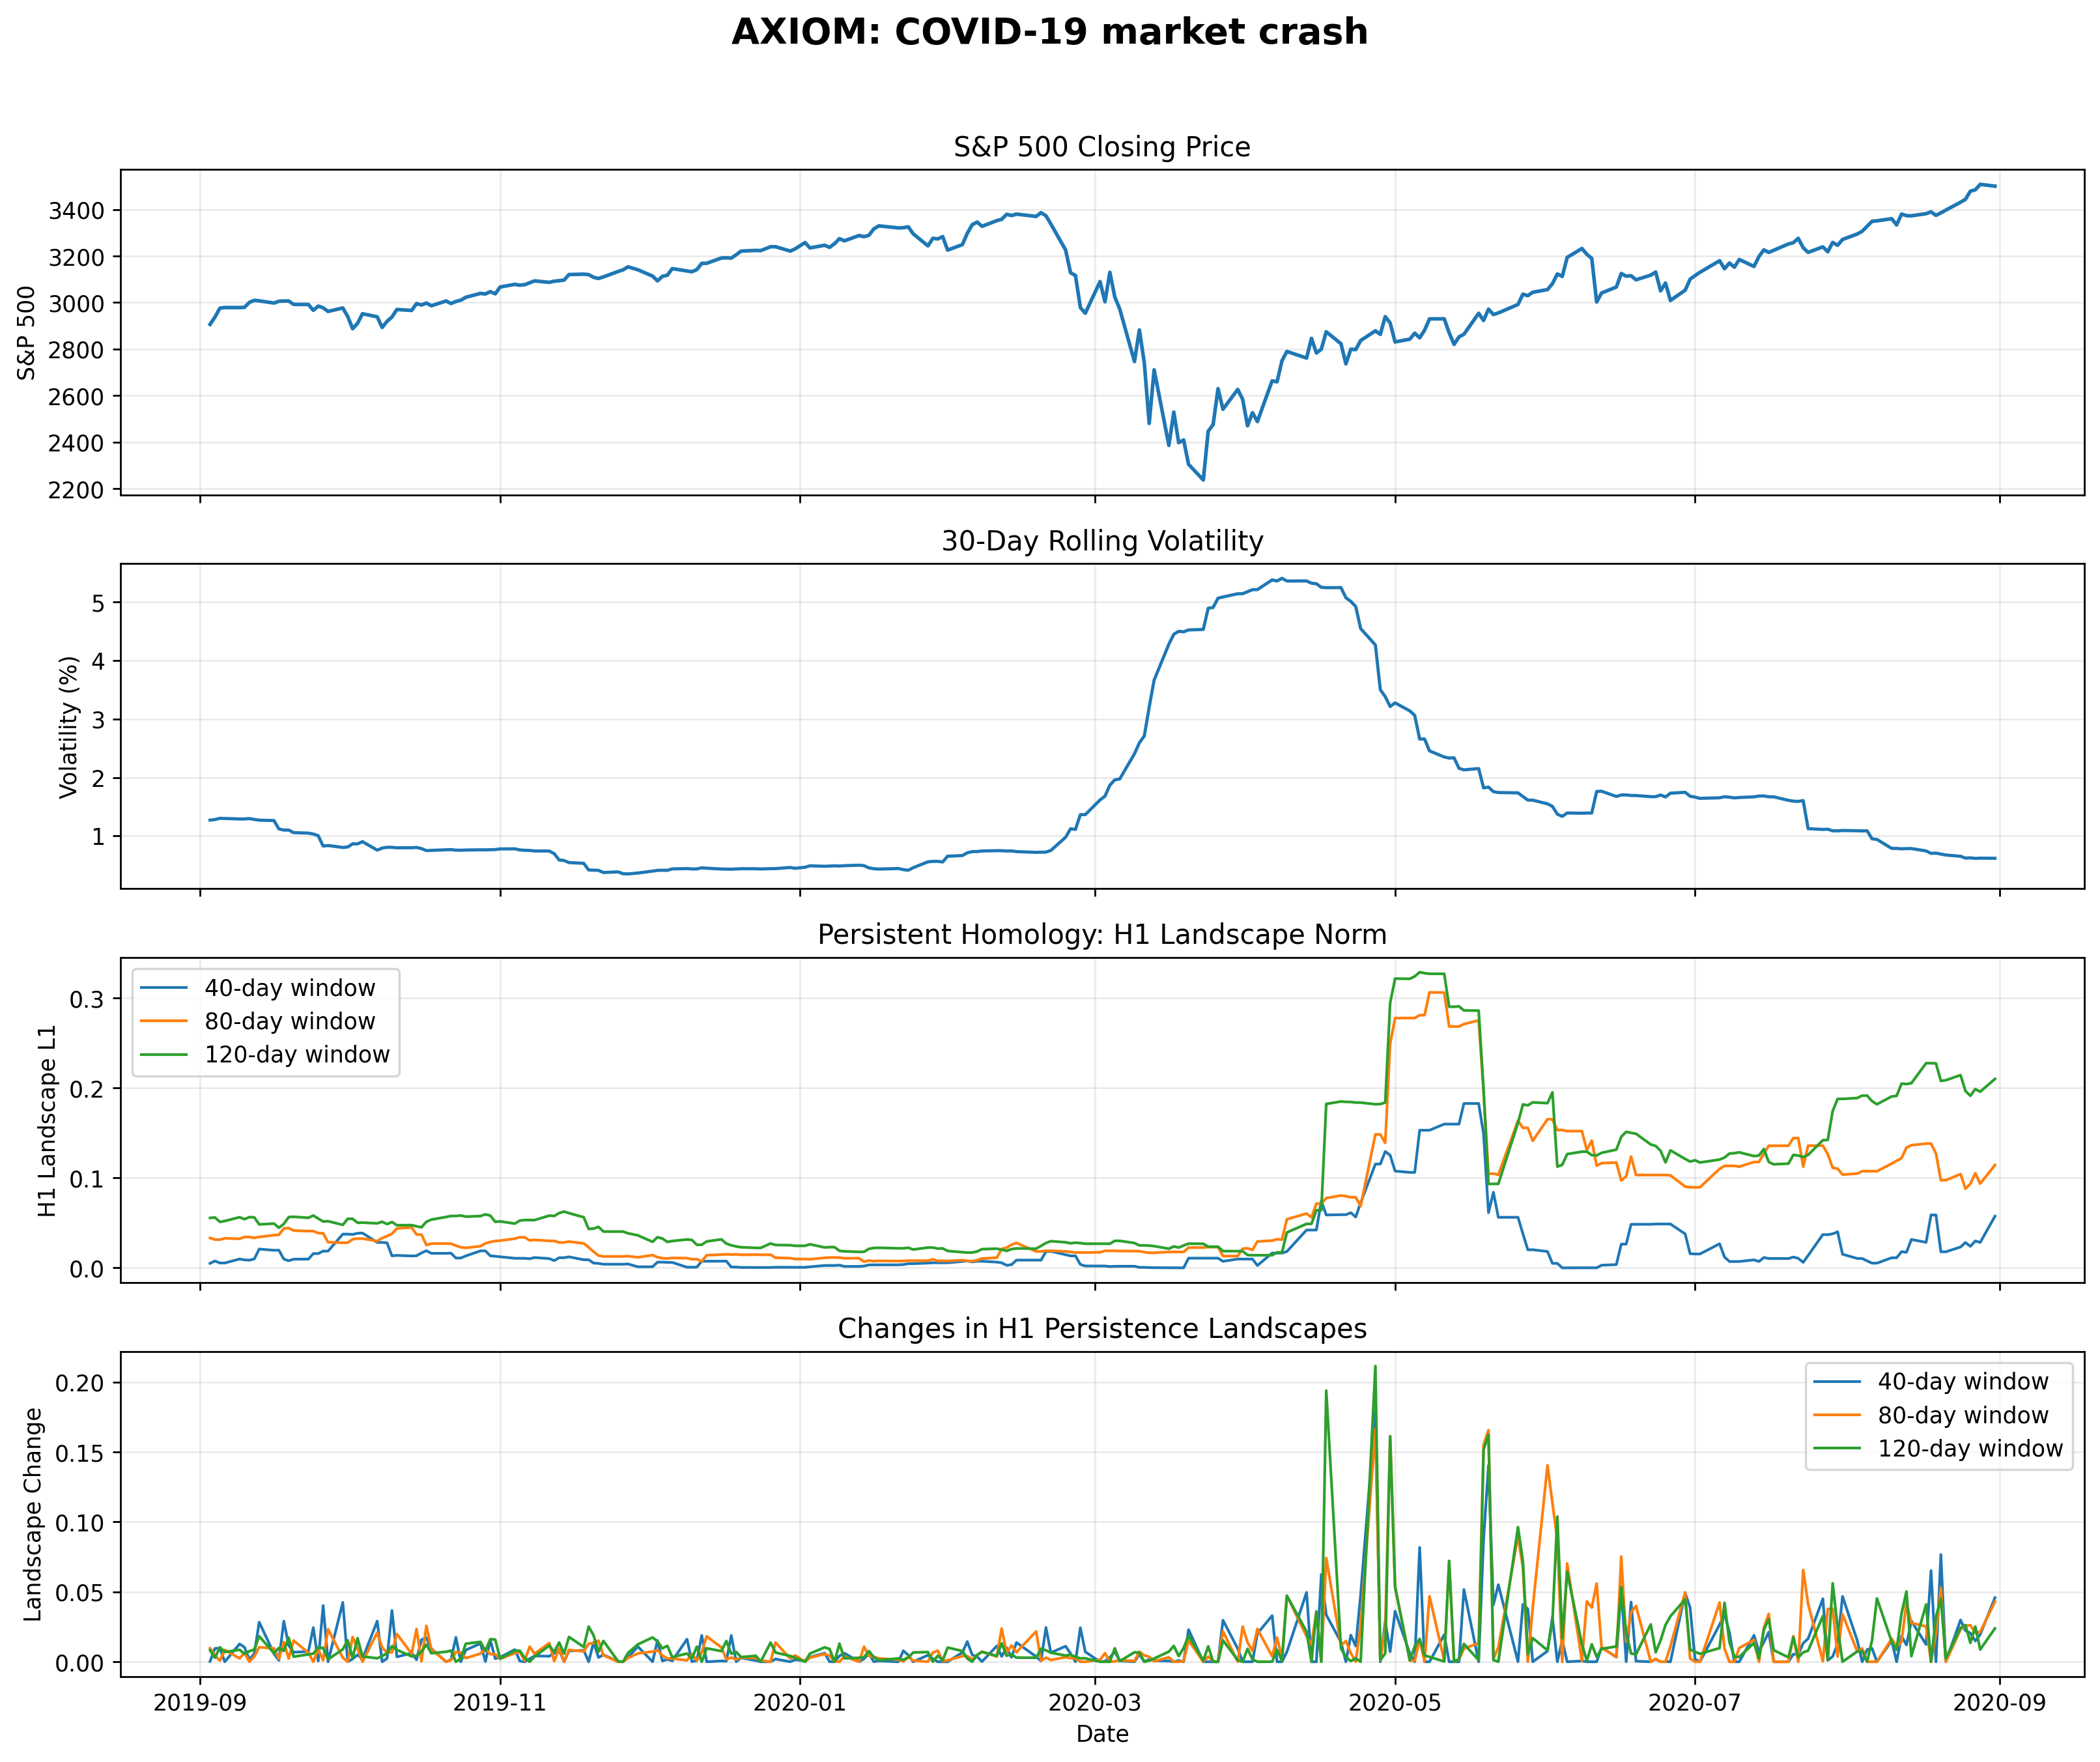
\includegraphics[
    width=0.88\textwidth,
    keepaspectratio
]{covid_19_market_crash.png}

\caption{
Classical volatility and topological indicators
around the COVID-19 market crash.
}

\label{fig:covid_crash}

\end{figure}

\FloatBarrier

\subsection{Saved-Model Prediction Demonstration}

For the prediction demonstration, I reload a previously trained checkpoint.

Both the model and its fitted scaler are restored without retraining. 

Model selection for the demonstration is based on validation average precision (AP). Specifically, the chosen checkpoint is a classical-feature LSTM with seed 42, which achieved a validation AP of 0.1173 and a test AP of 0.0852.

The configuration was selected by identifying the model with the highest mean validation AP among all compared setups, and then choosing the checkpoint with the best validation AP within that configuration. 

Although the combined-feature LSTM produced a higher mean test AP, test performance was not used for demonstration model selection. 

Therefore, the demonstration employs the classical-feature LSTM with seed 42. 

Note that its individual test AP of 0.0852 should not be conflated with the mean test AP of 0.1340 averaged across three random seeds.

The demonstration comprises 1,290 historical test observations, including 84 positive labels.

This serves as a historical prediction demonstration, not a live trading system.

\begin{figure}[htbp]
\centering

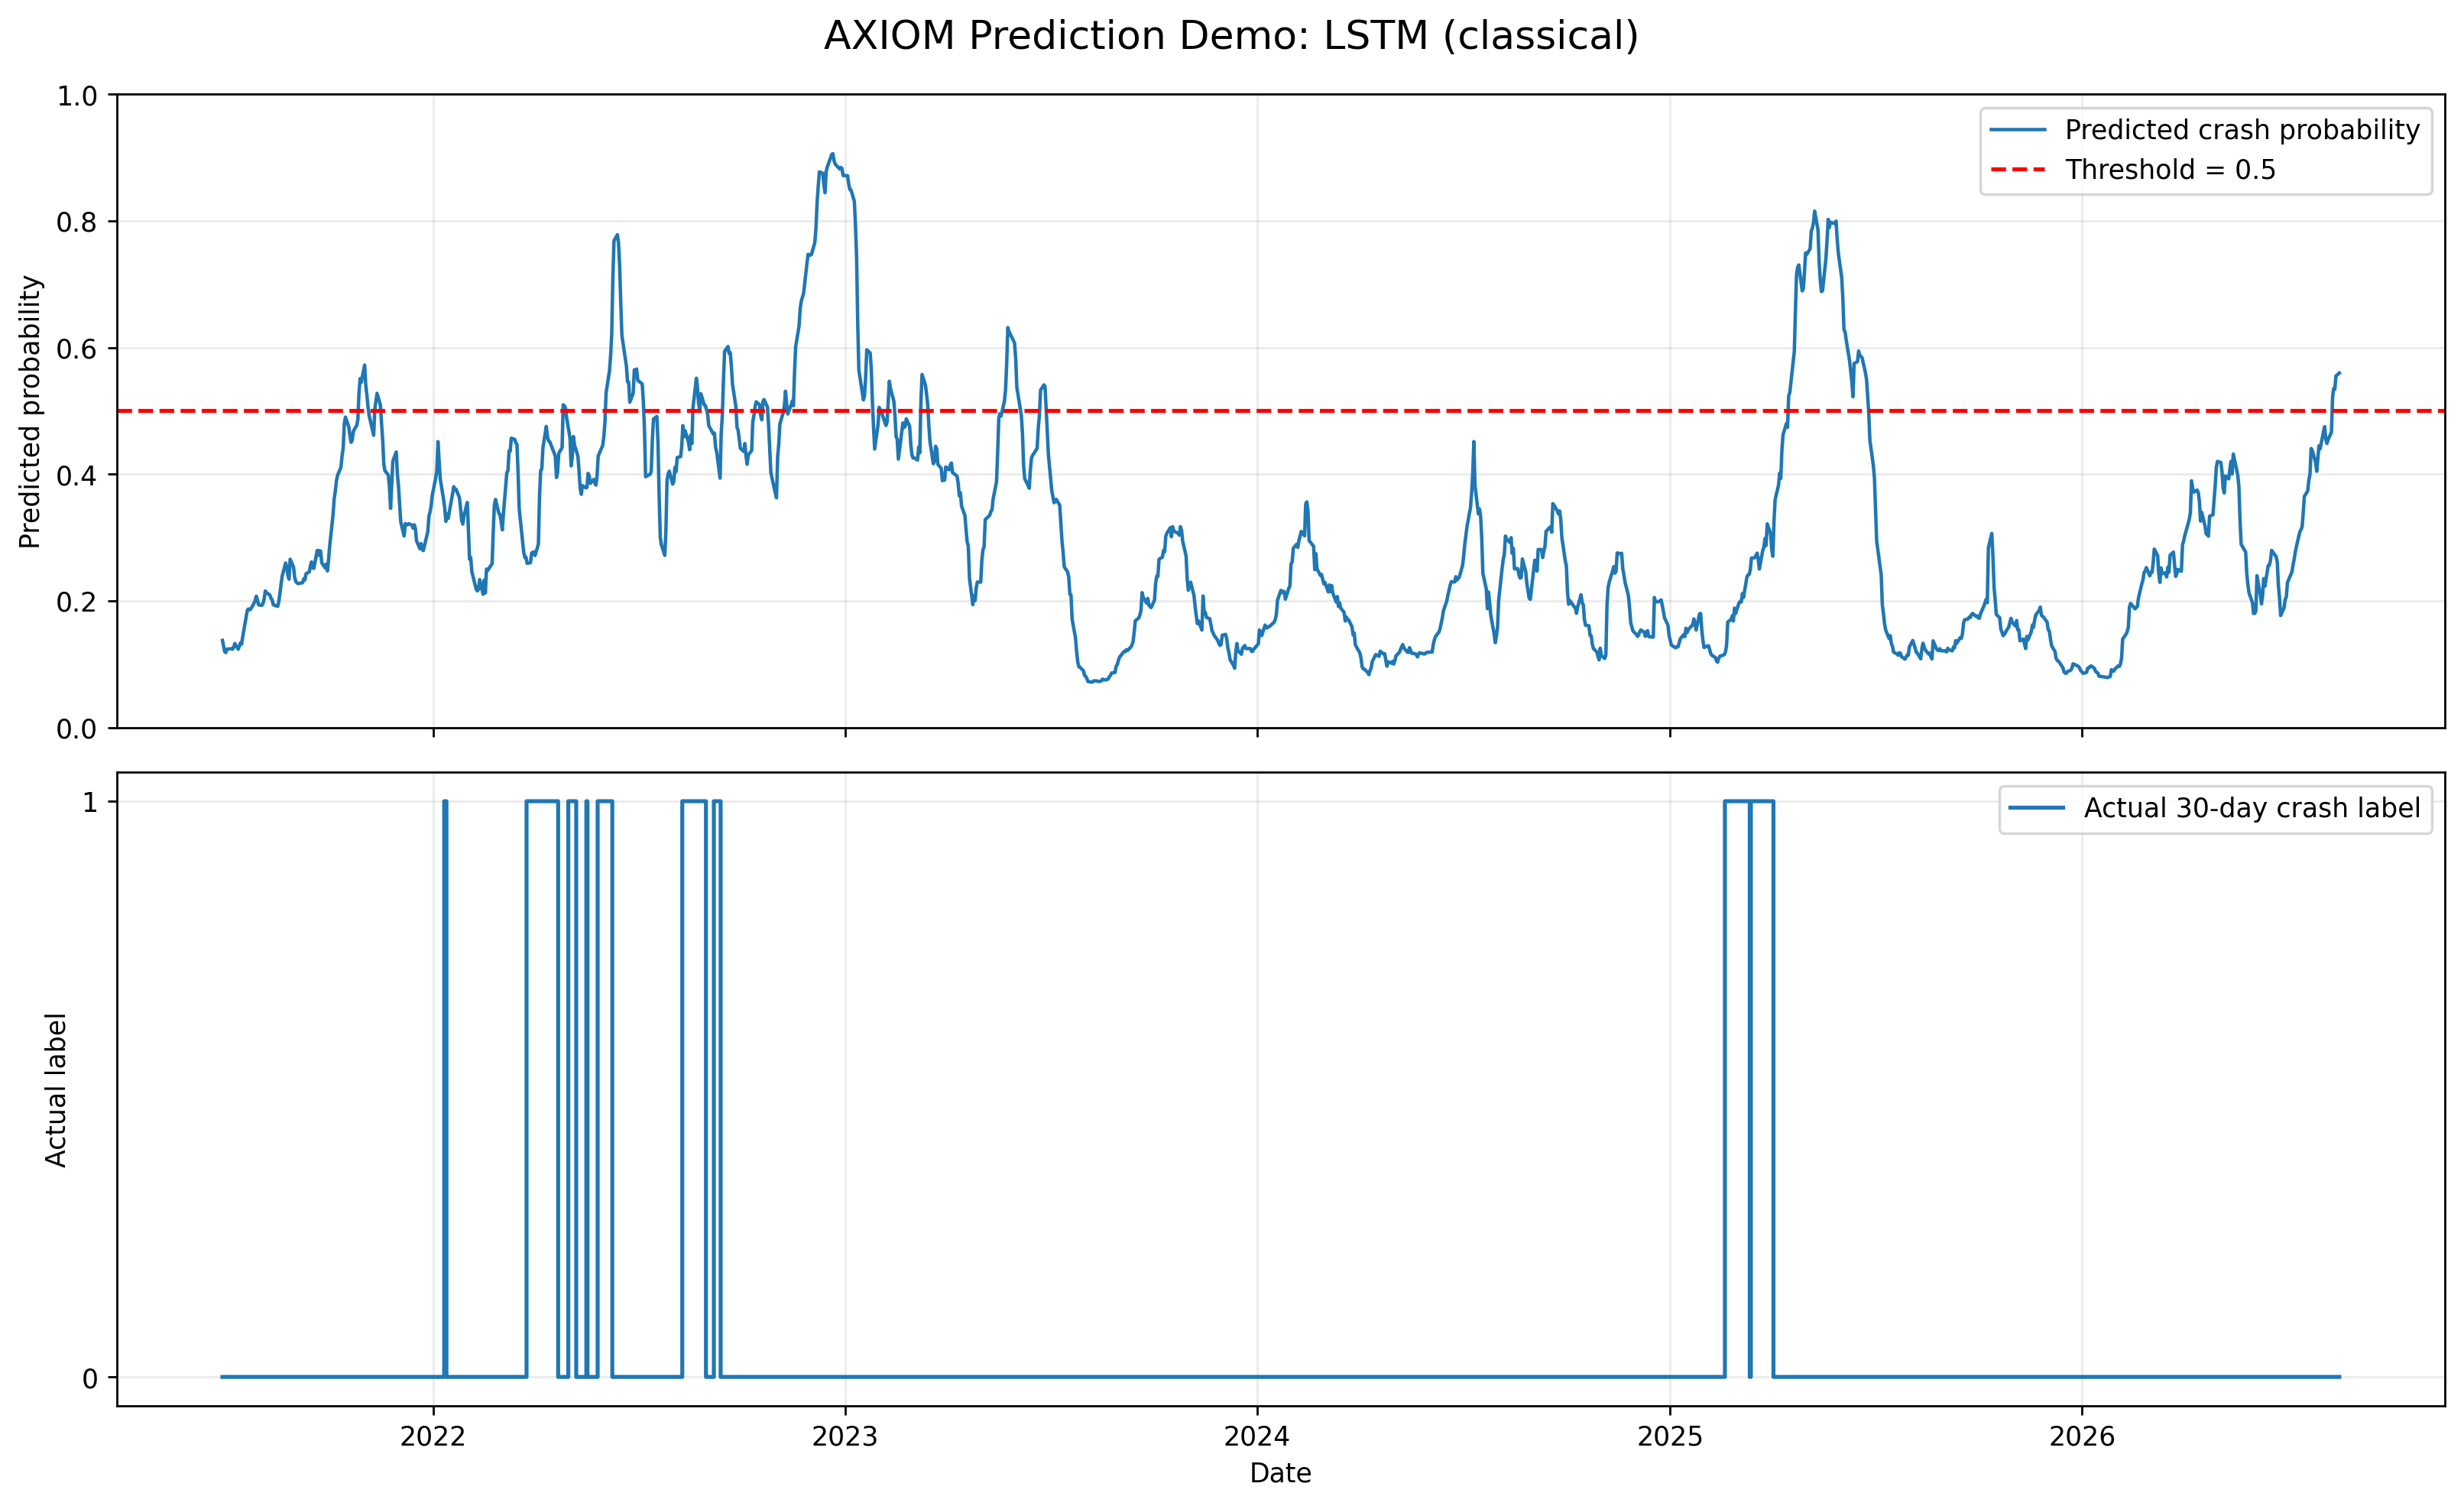
\includegraphics[
    width=0.88\textwidth,
    keepaspectratio
]{historical_prediction_demo.png}

\caption{
Historical crash-prediction scores
generated using the saved LSTM checkpoint.
}

\label{fig:prediction_demo}

\end{figure}

\FloatBarrier

\subsection{Limitations}

The experiments have several limitations. 

First, the return point clouds use Euclidean distances without standardizing each index coordinate separately before applying persistent homology, which may cause indices with larger return variability to dominate the geometry. 

Second, persistence landscapes are approximated using only five layers and 160 grid points, which may limit their resolution.

Third, only $H_0$ and $H_1$ homology groups are calculated, omitting higher-dimensional topological features.

Fourth, there is overlap between input sequences and future crash-label windows, as each crash label depends on the subsequent 30 trading days.

This overlap means that labels for nearby observations may rely on many of the same future prices, so consecutive test observations are not statistically independent.

The use of three random seeds measures variation due to model training, but all seeds rely on the same historical data and do not represent independent market samples.

Finally, the improvement of the combined LSTM on the test period is not reflected on the validation period, indicating inconsistent generalization. 

For these reasons, I interpret the results as an empirical comparison rather than definitive evidence of a robust early-warning system.



\section{Plan for Novelty Assessment}
\label{sec:novelty}

\subsection{What I Have Implemented}

The main objective of this project is to evaluate whether topological features can improve market crash prediction compared to classical financial indicators. Persistent homology and persistence landscapes are established mathematical tools
\citep{edelsbrunner2002,bubenik2015}
and previous research has applied these approaches to financial time series 
\citep{gidea2018,ismail2022}.

Therefore, this project does not introduce novel persistent-homology algorithms or deep learning architectures. Instead, the primary contribution is a systematic experimental comparison of existing methods on a unified crash-prediction task. Specifically, I:

\begin{enumerate}[leftmargin=*]

\item Constructed four-dimensional point clouds from daily returns of four stock indices

\item Extracted persistent-homology features using rolling windows of 40, 80, and 120 trading days

\item Compared three feature groups: classical financial indicators, topological features, and their combination

\item Trained logistic regression, LSTM, bidirectional LSTM, and Transformer models using chronological data splits

\item Repeated neural network experiments with three random seeds and varied TDA window sizes

\item Examined how topological features behave around historical market crashes

\end{enumerate}

These experiments enable a rigorous assessment of whether topological information provides independent predictive value when the prediction target, dataset, and evaluation method are controlled.


\subsection{What the Current Results Show}


The combined-feature LSTM achieved a mean test average precision of 0.2459, outperforming the classical-only LSTM, which scored 0.1340 on the same period.

While this indicates improvement on the selected test set, the mean validation average precision dropped from 0.1106 (classical LSTM) to 0.0690 (combined LSTM), suggesting that the added topological features do not consistently enhance crash prediction.

The window-size ablation revealed that combining all three TDA windows provided only a slightly higher mean test average precision than using any single window. 

Since the combined representation includes more features overall, the observed improvement cannot be attributed solely to the use of multiple time scales. 

These results indicate that the benefit of topological information may depend on both the specific market period and the chosen feature representation.


\subsection{How I Would Assess Novelty Further}

To determine whether the topological features provide information beyond what classical financial indicators capture, I would conduct the following additional experiments:

\begin{enumerate}[leftmargin=*]

\item \textbf{Walk-forward evaluation:}

Evaluate models across several non-overlapping historical test periods to assess if improvements persist under different market conditions.

\item \textbf{Timing of early-warning signals:}

Compare when topological and classical volatility indicators begin to change before historical crashes. An effective early-warning indicator should provide information ahead of a crash, not just react after the market falls.

\item \textbf{Effect of coordinate scaling:}

Repeat persistent-homology calculations after standardizing each of the four return coordinates separately. This clarifies whether topological features are mainly influenced by indices with higher return variability.

\item \textbf{Alternative distance metrics:}

Compare Euclidean distance with other suitable measures when constructing point clouds to examine sensitivity of topological features to the choice of distance metric.

\item \textbf{Stronger baseline comparisons:}

Compare combined-feature models with simpler models of similar capacity and well-tuned classical-feature baselines to ensure observed improvements stem from topological information, not just added model complexity.

\item \textbf{Prediction uncertainty:}

Study probability calibration and prediction stability across different historical periods to evaluate whether predicted crash probabilities can be interpreted reliably.

\end{enumerate}


\subsection{Scope of the Novelty Claim}

The present project does not introduce a new persistent-homology algorithm or neural network architecture. 

Its main contribution is the implementation and evaluation of a pipeline that combines topological and classical financial features for a well-defined crash-prediction task. 

While the current experiments provide evidence on the behavior of these feature groups, they are not sufficient to demonstrate a general improvement in forecasting performance. 

The additional experiments described above are necessary to make a stronger claim about the independent predictive value of topological features. 

These are proposed future experiments, not completed results.

\section{Conclusion}
\label{sec:conclusion}


In this project, I compared classical financial indicators with topological features for predicting market crashes.
Using daily returns from four major US stock indices, I constructed rolling point clouds to extract persistent-homology features.

I evaluated several models: logistic regression, LSTM, bidirectional LSTM, and Transformer architectures. The combined-feature LSTM achieved the highest mean test average precision (0.2459) among the neural network models, outperforming the classical-feature LSTM (0.1340).

However, the combined model underperformed on the validation period, indicating that the test improvement does not guarantee consistent generalization.

Window-size experiments also revealed a modest improvement when incorporating topological features from 40, 80, and 120 trading days. 

Overall, the results indicate that topological features may offer additional predictive value, but further evaluation across diverse market periods is necessary before drawing stronger conclusions.


\bibliographystyle{plainnat}
\bibliography{references}

\end{document}